\documentclass[tikz]{standalone}
\tikzset{near start abs/.style={xshift=1cm}}

\usetikzlibrary{positioning}
\begin{document}
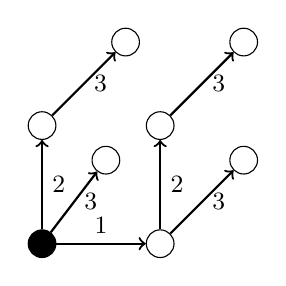
\begin{tikzpicture}[node distance=1.5cm]
    % place nodes
    \node[circle,draw=black, fill=black, inner sep=0pt,minimum size=10pt] (r) {};
    \node[circle,draw=black, fill=white, inner sep=0pt,right of=r, minimum size=10pt] (r1a)  {};
    \node[circle,draw=black, fill=white, inner sep=0pt,above right of=r, xshift=-0.25cm, minimum size=10pt] (r2a)  {};
    \node[circle,draw=black, fill=white, inner sep=0pt,above of=r, minimum size=10pt] (r2t)  {};
    \node[circle,draw=black, fill=white, inner sep=0pt,above right of=r2t, minimum size=10pt] (r3)  {};
    \node[circle,draw=black, fill=white, inner sep=0pt,above of=r1a, minimum size=10pt] (r2tb)  {};
    \node[circle,draw=black, fill=white, inner sep=0pt,above right of=r1a, minimum size=10pt] (r2tc)  {};
    \node[circle,draw=black, fill=white, inner sep=0pt,above right of=r2tb, minimum size=10pt] (r3tb)  {};
    % Arrows, right subgraph
    \draw[->,thick] (r) -- node[above] {\small{1}} ++(r1a);
    \draw[->,thick] (r1a) -- node[right] {\small{3}} ++(r2tc);
    \draw[->,thick] (r1a) -- node[right] {\small{2}} ++(r2tb);
    \draw[->,thick] (r2tb) -- node[right] {\small{3}} ++(r3tb);
    % Left subgraph
     \draw[->,thick] (r) -- node[right] {\small{3}} ++(r2a);
    \draw[->,thick] (r) -- node[right] {\small{2}} ++(r2t);
    \draw[->,thick] (r2t) -- node[right] {\small{3}} ++(r3);
\end{tikzpicture}
\end{document}